%%%%%%%%%%%%%%%%%%%%%%%%%%%%%%%%%%%%%%%%%
% eBook 
% LaTeX Template
% Version 1.0 (29/12/14)
%
% This template has been downloaded from:
% http://www.LaTeXTemplates.com
%
% Original author:
% Luis Cobo (luiscobogutierrez@gmail.com) with extensive modifications by:
% Vel (vel@latextemplates.com)
%
% License:
% CC BY-NC-SA 3.0 (http://creativecommons.org/licenses/by-nc-sa/3.0/)
%
%%%%%%%%%%%%%%%%%%%%%%%%%%%%%%%%%%%%%%%%%

%----------------------------------------------------------------------------------------
%	DOCUMENT CONFIGURATIONS AND INFORMATION
%----------------------------------------------------------------------------------------

\documentclass[14pt]{memoir} % Font size
%\documentclass[12pt]{memoir} % Font size A6


%----------------------------------------------------------------------------------------
%	GRAYSCALE EM TODAS AS FIGURAS
% Habilita o modo impressão em tons de cinza, não todo logicmente
% Mas a maioria das coisas, as figuras não, isto é para mandar à editora em GRAY SCALE
%----------------------------------------------------------------------------------------

%%% \def\EnableGrayScale{1}

%----------------------------------------------------------------------------------------
%	Muda La direccion raiz
%----------------------------------------------------------------------------------------
\def \SourceRootPath{.}


%----------------------------------------------------------------------------------------
%	DATOS DEL LIBRO
%----------------------------------------------------------------------------------------
\newcommand{\mytitle}[0]{Aulicha}
\newcommand{\mysubtitle}[0]{Cr\'onicas en los Andes}
\newcommand{\myauthor}[0]{Fernando Pujaico Rivera}
\newcommand{\imprimiredition}{Primera Edici\'on} % Book edition
%%% las aventuras de aulicha -crónicas en los andes (Mariano Pujaico Rivera)
%----------------------------------------------------------------------------------------

%----------------------------------------------------------------------------------------
%	DATOS PATROCINIO
%----------------------------------------------------------------------------------------
\newcommand{\ImprimirLinkGitHub}[0]{https://trucomanx.github.io}%{https://localhost}%{https://trucomanx.github.io}
\newcommand{\ImprimirLinkHomePageLivro}[0]{\url{\ImprimirLinkGitHub/aulicha}}

%----------------------------------------------------------------------------------------
%   Tamanho da folha
%----------------------------------------------------------------------------------------
%%\def \imprimirpagewidthcm{10.5}  %% A6 
%%\def \imprimirpageheightcm{14.8} %% A6
\def \imprimirpagewidthcm{14.8}  %% A5 
\def \imprimirpageheightcm{21.0} %% A5
%% \def \imprimirpagewidthcm{21.0}  %% A4 
%% \def \imprimirpageheightcm{29.7} %% A4


%----------------------------------------------------------------------------------------
%   DADOS ficha catalográfica
%----------------------------------------------------------------------------------------
\def \myauthorname{Fernando}
\def \myauthorlastname{Pujaico Rivera}
\def \myauthorborn{1982}
\def \imprimirlocal{Lavras}%cidade obrigatorio
\def \imprimiryear{2020}
\newcommand{\imprimirdata}[0]{agosto de \imprimiryear}
\def \imprimirtipotrabalho{Incluye Bibliograf\'ia}
\def \imprimirISNI{\href{http://isni.org/isni/000000049156373X}{0000 0004 9156 373X}}
\def \imprimirOrcid{\url{https://orcid.org/0000-0002-4970-2818}}
\def \imprimircuttersanborn{\textcolor{red}{P979X}} %% Nome+titulo %% https://www.cuttersonline.com/app/generator/?q=Pujaico&ref=sanborn&add=
\newcommand{\imprimirpapersize}[0]{{\imprimirpagewidthcm}x{\imprimirpageheightcm}cm}%%{21x30cm}
\def \imprimirCDD{028.5}        %% 028.5 - conto infantil                  %% https://books.google.com.br/books?id=G2xHIl0suOcC&pg=PP46&dq=conto+infantil+cdd&hl=pt-BR&sa=X&ved=2ahUKEwiVq_un6ZnrAhWgILkGHSBeCQkQ6AEwBHoECAEQAg#v=onepage&q=conto%20infantil%20cdd&f=false
                                                                           %% https://books.google.com.br/books?id=bAxcCgAAQBAJ&pg=PA2&dq=conto+infantil+cdd&hl=pt-BR&sa=X&ved=2ahUKEwiVq_un6ZnrAhWgILkGHSBeCQkQ6AEwAnoECAUQAg#v=onepage&q=conto%20infantil%20cdd&f=false
                                %% 808 - Coleções de Literatura e Retórica %% http://bilica.org.br/sistema/modulos/acervo/cdd.php?codigo=800#800
                                %% 808.899282 - LITERATURA INFANTIL        %% http://www.biblivre.org.br/forum/viewtopic.php?f=87&t=3097
                                                                           %% https://www.oclc.org/content/dam/oclc/dewey/updates/ddc23/808.8Manual_20130329_DDC%2023.pdf
                                %% 898 - Nativas das América do Sul        %% http://bilica.org.br/sistema/modulos/acervo/cdd.php?codigo=890#800
\def \imprimirCDU{087.5}        %% Publicações para jovens e infantis      %% https://bibliotextos.files.wordpress.com/2014/07/cdu-parte-i.pdf
\newcommand{\imprimirisbn}[0]{\textcolor{red}{XXX-XX-XX-XXXXX-X}}
\def \imprimireditora{Edici\'on Independiente}%%{Autopublica\c{c}\~{a}o}%%{Edi\c{c}\~{a}o Independente}
\def \palavraschavea{Cuento infantil}
\def \palavraschaveb{Cuento peruano}
\def \palavraschavec{Literatura Latino-Americana}
\def \palavraschavesInglesa{children's tale}
\def \palavraschavesInglesb{Peruvian tale}
\def \palavraschavesInglesc{Latin American Literature}
%----------------------------------------------------------------------------------------


%----------------------------------------------------------------------------------------
%	XCOLOR
%----------------------------------------------------------------------------------------
\usepackage[dvipsnames*,svgnames]{xcolor}

\definecolor{colorlowgray}{RGB}{240,240,240}

%----------------------------------------------------------------------------------------
%	COLOR
%----------------------------------------------------------------------------------------
\usepackage{color}

%----------------------------------------------------------------------------------------

%----------------------------------------------------------------------------------------
%----------------------------------------------------------------------------------------
%----------------------------------------------------------------------------------------
%%%%%%%%%%%%%%%%%%%%%%%%%%%%%%%%%%%%%%%%%
% eBook
% Structural Definitions File
% Version 1.0 (29/12/14)
%
% Created by:
% Vel (vel@latextemplates.com)
% 
% This file has been downloaded from:
% http://www.LaTeXTemplates.com
%
% License:
% CC BY-NC-SA 3.0 (http://creativecommons.org/licenses/by-nc-sa/3.0/)
%
%%%%%%%%%%%%%%%%%%%%%%%%%%%%%%%%%%%%%%%%%

%----------------------------------------------------------------------------------------
%	REQUIRED PACKAGES
%----------------------------------------------------------------------------------------

%----------------------------------------------------------------------------------------
%	ACENTOS
%----------------------------------------------------------------------------------------
\usepackage[utf8]{inputenc} % Required for including letters with accents
\usepackage[T1]{fontenc} % Use 8-bit encoding that has 256 glyphs
\usepackage[spanish]{babel}
%----------------------------------------------------------------------------------------

\usepackage{lipsum} % Inserts dummy text

%----------------------------------------------------------------------------------------
%	VARIOUS REQUIRED PACKAGES AND CONFIGURATIONS
%----------------------------------------------------------------------------------------

\usepackage{graphicx} % Required for including pictures
\graphicspath{{\SourceRootPath/pictures/}} % Specifies the directory where pictures are stored


%----------------------------------------------------------------------------------------
% Par diferentes modelos de caption.
%----------------------------------------------------------------------------------------
\usepackage{caption}
\usepackage{subcaption}
\usepackage{wrapfig}
%----------------------------------------------------------------------------------------

%----------------------------------------------------------------------------------------
% ROTATION FIGURE
%----------------------------------------------------------------------------------------
% For rotating figures, tables, etc.
%  including their captions
% \begin{sidewaysfigure}[ht]
% \end{sidewaysfigure}
\usepackage[figuresleft]{rotating}
%----------------------------------------------------------------------------------------


%----------------------------------------------------------------------------------------
% Page counter
%----------------------------------------------------------------------------------------
\usepackage{lastpage}
%----------------------------------------------------------------------------------------

%----------------------------------------------------------------------------------------
\usepackage{paralist} %% \begin{inparaenum}
%----------------------------------------------------------------------------------------

%----------------------------------------------------------------------------------------
% Para \singlespacing 
%----------------------------------------------------------------------------------------
\usepackage{setspace}
%----------------------------------------------------------------------------------------

\usepackage[osf]{libertine} % Use the Libertine font
\usepackage{microtype} % Improves character and word spacing

\usepackage{tikz} % Required for drawing custom shapes
\definecolor[named]{color01}{rgb}{.2,.4,.6} % Color used in the title page
\usepackage{wallpaper} % Required for setting background images (title page)

\usepackage[unicode=true,bookmarks=true,bookmarksnumbered=false,bookmarksopen=false,breaklinks=false,pdfborder={0 0 1},backref=section,colorlinks=false]{hyperref} % PDF meta-information specification

%----------------------------------------------------------------------------------------
%	PAPER, MARGIN AND HEADER/FOOTER SIZES
%----------------------------------------------------------------------------------------

\setstocksize{{\imprimirpageheightcm}cm}{{\imprimirpagewidthcm}cm} % Paper size A6
\settrimmedsize{\stockheight}{\stockwidth}{*} % No trims
\setlrmarginsandblock{60pt}{60pt}{*} % Left/right margins
\setulmarginsandblock{60pt}{60pt}{*} % Top/bottom margins
\setheadfoot{28pt}{36pt} % Header/footer height
\setheaderspaces{*}{8pt}{*} % Extra header space

%----------------------------------------------------------------------------------------
%	FOOTNOTE CUSTOMIZATION
%----------------------------------------------------------------------------------------

\renewcommand{\foottextfont}{\itshape\footnotesize} % Font settings for footnotes
\setlength{\footmarkwidth}{-.1em} % Space between the footnote number and the text
\setlength{\footmarksep}{.1em} % Space between multiple footnotes on the same page
\renewcommand*{\footnoterule}{} % Remove the rule above the first footnote
\setlength{\skip\footins}{1\onelineskip} % Space between the body text and the footnote

%----------------------------------------------------------------------------------------
%	HEADER AND FOOTER FORMATS
%----------------------------------------------------------------------------------------

\makepagestyle{mio} % Define a new custom page style
\setlength{\headwidth}{\textwidth} % Header the same width as the text
\makeheadrule{mio}{\textwidth}{0.1mm} % Header rule height
\makeoddhead{mio}{\scriptsize{\theauthor\hskip.2cm\vrule\hskip.2cm\itshape{\thetitle}}}{}{} % Header specification
\makeoddfoot{mio}{}{\scriptsize {\thepage \quad \vrule \quad \thelastpage}}{} % Footer specification
\makeoddfoot{plain}{}{\footnotesize {\thepage \quad \vrule \quad \thelastpage}}{} % Pages of chapters
\pagestyle{mio} % Set the page style to the custom style defined above

%----------------------------------------------------------------------------------------
%	PART FORMAT
%----------------------------------------------------------------------------------------

\renewcommand{\partnamefont}{\centering\sffamily\itshape\Huge} % Part name font specification
\renewcommand{\partnumfont}{\sffamily\Huge} % Part number font specification
\renewcommand{\parttitlefont}{\centering\sffamily\scshape} % Part title font specification
\renewcommand{\beforepartskip}{\null\vskip.618\textheight} % Whitespace above the part heading

%----------------------------------------------------------------------------------------
%% background of part
\makeatletter
% define a user command to choose the image
% this command also creates an internal command to insert the image
\newcommand{\partimage}[2][]{\gdef\@partimage{\ThisCenterWallPaper{#1}{#2} }}
\renewcommand{\printparttitle}[1]{\parttitlefont #1\vfil\@partimage\vfil}
\makeatother

%----------------------------------------------------------------------------------------
%	CHAPTER FORMAT
%----------------------------------------------------------------------------------------

\makechapterstyle{Tufte}{ % Define a new chapter style
\renewcommand{\chapterheadstart}{\null \vskip3.5\onelineskip} % Whitespace before the chapter starts
\renewcommand{\printchaptername}{\large\itshape\chaptername} % "Chapter" text font specification
\renewcommand{\printchapternum}{\LARGE\thechapter \\} % Chapter number font specification
\renewcommand{\afterchapternum}{} % Space between the chapter number and text
\renewcommand{\printchaptertitle}[1]{ % Chapter title font specification
\raggedright
\itshape\Huge{##1}}
\renewcommand{\afterchaptertitle}{
\vskip3.5\onelineskip
}}
\chapterstyle{Tufte} % Set the chapter style to the custom style defined above

%----------------------------------------------------------------------------------------
%	SECTION FORMAT
%----------------------------------------------------------------------------------------

\setsecheadstyle{\sethangfrom{\noindent ##1}\raggedright\sffamily\itshape\Large} % Section title font specification
\setbeforesecskip{-.6\onelineskip} % Whitespace before the section
\setaftersecskip{.3\onelineskip} % Whitespace after the section

%----------------------------------------------------------------------------------------
%	SUBSECTION FORMAT
%----------------------------------------------------------------------------------------

\setsubsecheadstyle{\sethangfrom{\noindent  ##1}\raggedright\sffamily\large\itshape} % Subsection title font specification
\setbeforesubsecskip{-.5\onelineskip} % Whitespace before the subsection
\setaftersubsecskip{.2\onelineskip} % Whitespace after the subsection

%----------------------------------------------------------------------------------------
%	SUBSUBSECTION FORMAT
%----------------------------------------------------------------------------------------

\setsubsubsecheadstyle{\sethangfrom{\noindent ##1}\raggedright\sffamily\itshape} % Subsubsection title font specification
\setbeforesubsubsecskip{-.5\onelineskip} % Whitespace before the subsubsection
\setaftersubsubsecskip{.1\onelineskip} % Whitespace after the subsubsection

%----------------------------------------------------------------------------------------
%	CAPTION FORMAT
%----------------------------------------------------------------------------------------

\captiontitlefont{\itshape\footnotesize} % Caption font specification
\captionnamefont{\footnotesize} % "Caption" text font specification

%----------------------------------------------------------------------------------------
%	QUOTATION ENVIRONMENT FORMAT
%----------------------------------------------------------------------------------------

\renewenvironment{quotation}
{\par\leftskip=1em\vskip.5\onelineskip\em}
{\par\vskip.5\onelineskip}

%----------------------------------------------------------------------------------------
%	QUOTE ENVIRONMENT FORMAT
%----------------------------------------------------------------------------------------

\renewenvironment{quote}
{\list{}{\em\leftmargin=1em}\item[]}{\endlist\relax}


%----------------------------------------------------------------------------------------
%	CONTENTS TABLE
%----------------------------------------------------------------------------------------
% \usepackage{tocloft}
% \cftsetindents{chapter}{2em}{2em}
%----------------------------------------------------------------------------------------
\usepackage{titletoc}
% %% \dottedcontents{<section>}[<left>]{<above-code>}{<label width>}{<leader width>}
% \dottedcontents{part}[3em]{\bfseries }{2.9em}{1pc}
\dottedcontents{chapter}[2.9em]{\bfseries}{2.9em}{1pc}

%----------------------------------------------------------------------------------------
%	NO reiniciar la cuenta de paginas en \mainmatter
%----------------------------------------------------------------------------------------
\makeatletter
\def\pagenumbering#1{%
  \gdef\thepage{\csname @#1\endcsname \c@page}}
\makeatother
%----------------------------------------------------------------------------------------
%	MISCELLANEOUS DOCUMENT SPECIFICATIONS
%----------------------------------------------------------------------------------------

\setlength{\parindent}{1em} % Paragraph indentation

\midsloppy % Fewer overfull lines - used in the memoir class and allows a setting somewhere between \fussy and \sloppy

\checkandfixthelayout % Tell memoir to implement the above
 % el estilo visual do livro

%----------------------------------------------------------------------------------------
%  footnote font size
%----------------------------------------------------------------------------------------
\renewcommand{\footnotesize}{\small}

%----------------------------------------------------------------------------------------
%	Horizontal separator line
%   \HRule{2pt}
%----------------------------------------------------------------------------------------
\newcommand{\HRule}[1]{\rule{\linewidth}{#1}} % creo el comando  \HRule regla horizontal



%----------------------------------------------------------------------------------------
%	Horizontal separator line
%   \PRLsep{Text}
%----------------------------------------------------------------------------------------
\newlength{\PRLlen}
\newcommand*\PRLsep[1]{\settowidth{\PRLlen}{#1}\advance\PRLlen by -\textwidth\divide\PRLlen by -2\noindent\makebox[\the\PRLlen]{\resizebox{\the\PRLlen}{1pt}{$\blacktriangleleft$}}\raisebox{-.5ex}{\textbf{#1}}\makebox[\the\PRLlen]{\resizebox{\the\PRLlen}{1pt}{$\blacktriangleright$}}\bigskip}


%----------------------------------------------------------------------------------------
%----------------------------------------------------------------------------------------
%----------------------------------------------------------------------------------------
%----------------------------------------------------------------------------------------
% BOX - TCOLORBOX
%----------------------------------------------------------------------------------------
\usepackage[most,many]{tcolorbox}
\usetikzlibrary{decorations.pathmorphing}
\tcbuselibrary{skins}


%%%%%%%%%%%%%%%%%%%%%%%%%%%%%%%%%%%%%%%%%%%%%%%%%%%%%%%%%%%%%%%%%%%%%%%%%%%%%%%%
%%%%%%%%%%%%%%%%%%%%%%%%%%%%%%%%%%%%%%%%%%%%%%%%%%%%%%%%%%%%%%%%%%%%%%%%%%%%%%%%
%%%%%%%%%%%%%%%%%%%%%%%%%%%%%%%%%%%%%%%%%%%%%%%%%%%%%%%%%%%%%%%%%%%%%%%%%%%%%%%%
%%%%%%%%%%%%%%%%%%%%%%%%%%%%%%%%%%%%%%%%%%%%%%%%%%%%%%%%%%%%%%%%%%%%%%%%%%%%%%%%
%% UN SOLO USO
%%%%%%%%%%%%%%%%%%%%%%%%%%%%%%%%%%%%%%%%%%%%%%%%%%%%%%%%%%%%%%%%%%%%%%%%%%%%%%%%


%----------------------------------------------------------------------------------------
% CATALOGRAFICA MESSAGE BOX
%----------------------------------------------------------------------------------------
% \begin{catalografica}
%   texto
% \end{catalografica}

\newtcolorbox{catalografica}
{
  breakable,
  enhanced,
  arc=0mm,
  width=\textwidth,
  colback  = white,
  colframe = black
}

 % las macros compuestas usadas para la escrita
%----------------------------------------------------------------------------------------

\hyphenation{zan-dor}
\hyphenation{zo-rra}
\hyphenation{A-ya-cu-cho}

%-----------------------------------------------------------------------------------------
% evitar linhas órfãs e viúvas
\clubpenalty=100000 
\widowpenalty=100000 
%-----------------------------------------------------------------------------------------

%----------------------------------------------------------------------------------------
% Agrega marca de agua a cada pagina do livro
%----------------------------------------------------------------------------------------
\begin{comment}
\usepackage{draftwatermark}
\SetWatermarkText{Preview-Preview}
\SetWatermarkColor[gray]{0.9}
\SetWatermarkScale{1}
\end{comment}
%-----------------------------------------------------------------------------------------

\title{\mytitle} % Book title
\author{\myauthor} % Author


%----------------------------------------------------------------------------------------
%	My macros
%----------------------------------------------------------------------------------------
\makeatletter
\newcommand{\showfont}{codifica\c{c}\~ao: \f@encoding{},
  familia: \f@family{},
  serie: \f@series{},
  %shape: \f@shape{},
  e tamanho: \f@size{} pt
}



\newcommand{\AulichaEdad}{10}
\newcommand{\AulichaAnho}{1930} 


%----------------------------------------------------------------------------------------

\begin{document}

\frontmatter
%----------------------------------------------------------------------------------------
%	TITLE PAGE
%----------------------------------------------------------------------------------------
\cleardoublepage
\newpage
\thispagestyle{empty}

%% \begin{comment}
\begin{titlepage}
\begin{center}
%% Upper part of the page
%\includegraphics[width=1\textwidth]{./up-logo.jpg}\\[0.4cm]    
\textsc{\LARGE Primeira Edição}\\[0.25cm]
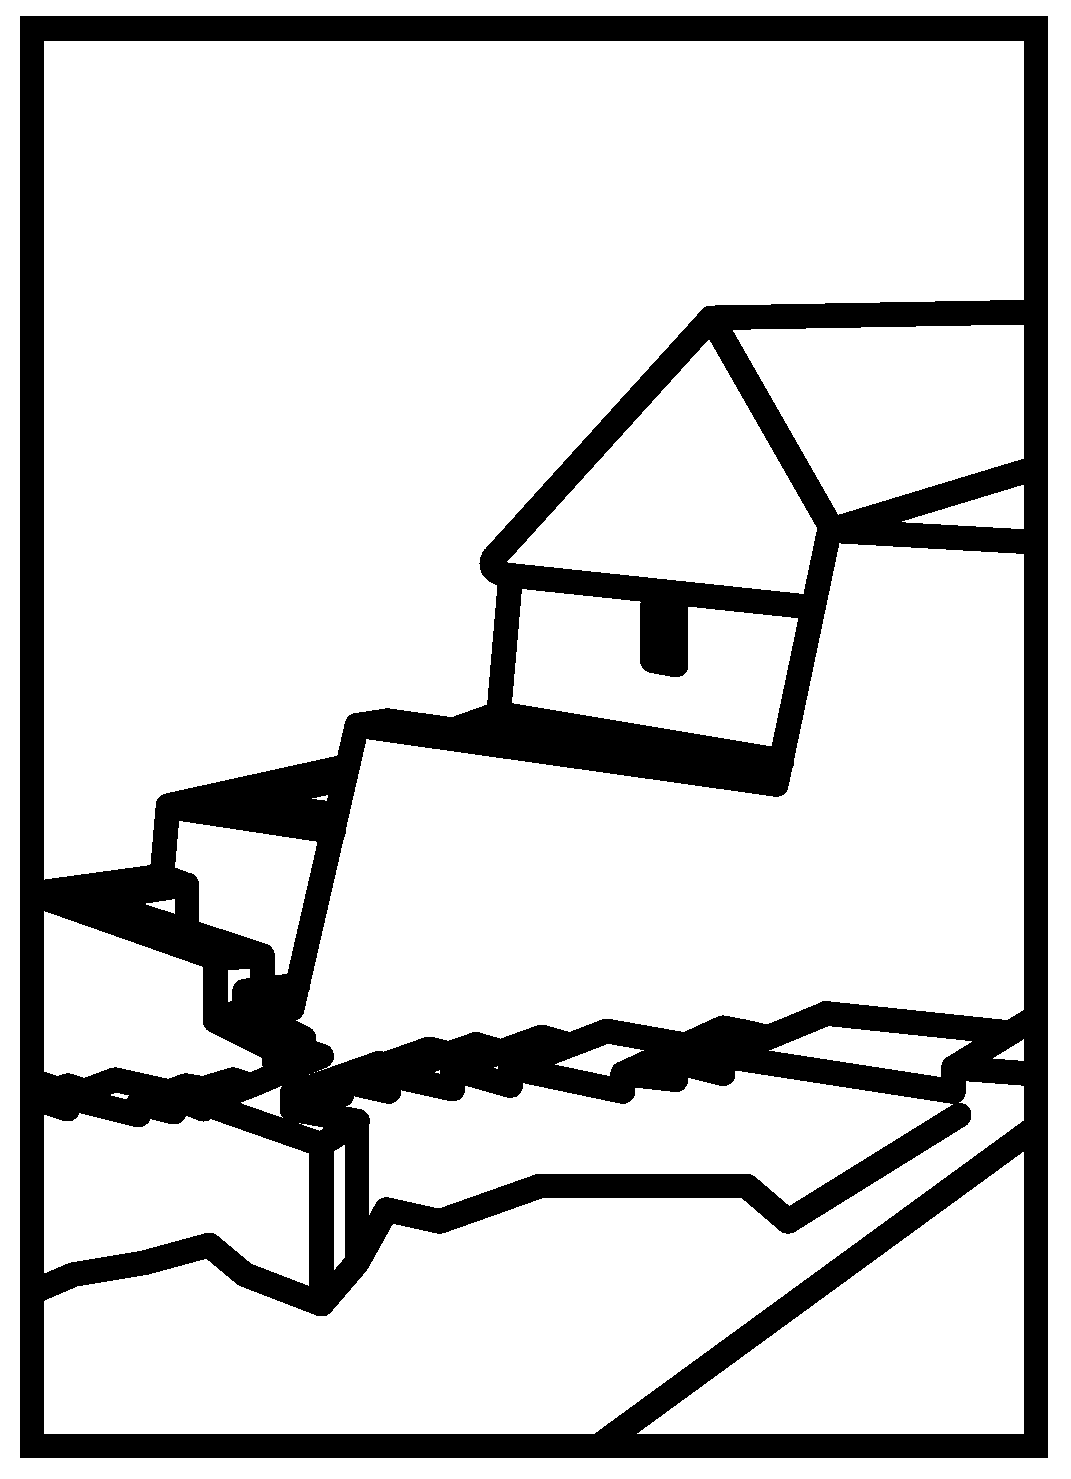
\includegraphics[width=0.25\textwidth]{principal}\\[0.25cm]
%% pretitle
%{\fontsize{25}{30} \textsc{Algum pretitulo}}
%% Title
\HRule{0.4cm} \\[0.4cm]
{ \huge \bfseries \mytitle}\\[0.4cm]
\HRule{0.4cm} \\[0.7cm]
%% SubTitle
{\LARGE \textsc{\mysubtitle}}\\[0.5cm]
\vfill
%% Author 
\textsc{\Large  \myauthor }
\begin{comment}
\begin{minipage}{0.4\textwidth}
\begin{flushleft} \large
%\emph{Author:}\\
\myauthor %\textsc{Coppejans}
\end{flushleft}
\end{minipage}
% ID
\begin{minipage}{0.4\textwidth}
\begin{flushright} \large
\emph{email:} \\
\ImprimirEmail
\end{flushright}
\end{minipage}
\end{comment}
% Bottom of the page
\vfill
\textsc{\Large Lavras/MG}\\[0.4cm]
\textsc{\Large \imprimiryear}
\end{center}
\end{titlepage}
%% \end{comment}


%----------------------------------------------------------------------------------------
%	COPYRIGHT PAGE
%----------------------------------------------------------------------------------------
%\cleardoublepage

\newpage
\thispagestyle{empty}

{\fontsize{0.035\textwidth}{0}

\noindent Copyright \copyright\ \imprimiryear\ \myauthor\\ % Copyright notice
\noindent \textbf{ISNI  ::} \imprimirISNI\\
\noindent \textbf{ORCID ::} \imprimirOrcid\\
~\\
\noindent \textbf{ISBN:} \imprimirisbn\\ % Publisher
\noindent \textbf{Publicado:} \imprimireditora\\ % Publisher
\noindent \textbf{Primeira impressão:} \imprimiryear\\ % Printing/edition date
\noindent \textbf{Diagramação:} \myauthor\\ % Printing/edition date
\noindent \textbf{Revisão de texto:} \textcolor{red}{XXXXXX XXXXXX}\\ % Printing/edition date
\noindent \textbf{Capa:} \myauthor\\ % Printing/edition date
\noindent \textbf{Página web:} \ImprimirLinkHomePageLivro\\ % Printing/edition date
~\\
\begin{center}
\begin{catalografica}%%
	\myauthorlastname, \myauthorname, \myauthorborn.%Sobrenome, Nome do autor

	\hspace{0.5cm} \mytitle: \mysubtitle~/ \myauthor. -- %\mytitle inicia na quarta letra do sobrenome
	\imprimirlocal, \imprimireditora, \imprimiryear.
	
	\hspace{0.5cm} \pageref{LastPage} p.: \imprimirpapersize.\\ %: il. (algumas color.) ; \imprimirpapersize.
	
	\hspace{0.5cm}
	\parbox[t]{\textwidth}{\imprimirtipotrabalho}%~--~\imprimireditora,~\imprimirdata.}\\

	\hspace{0.5cm}
	\parbox[t]{\textwidth}{ISBN: \imprimirisbn}\\


	\hspace{0.5cm}
	\begin{inparaenum}[1.]
		\item \palavraschavea.
		\item \palavraschaveb.
		\item \palavraschavec.
	\end{inparaenum}
	\begin{inparaenum}[I.]
		\item Título.% O livro deve ser encontrado pelo titulo
	\end{inparaenum}

    \begin{flushright}
    CDD: \imprimirCDD\\
    CDU: \imprimirCDU
    \end{flushright}
\end{catalografica}%%
\end{center}

}


%----------------------------------------------------------------------------------------
%	DEDICATORIA
%----------------------------------------------------------------------------------------
\cleardoublepage

\null
\vfill
\thispagestyle{empty}



{\normalsize \it \hfill Dedico este livro 
a meu pai Aurelio Pujaico Osccorima, 
a minha mãe Flaviana Rivera Illanes
e a meu irmão Mariano Pujaico Rivera.  \vspace*{4pt}}
 

%----------------------------------------------------------------------------------------
%	Acknowledgements
%----------------------------------------------------------------------------------------
\cleardoublepage

\begin{center}
\Huge{\textbf{Agradecimentos}}
\end{center}

\null
\vfill
\thispagestyle{empty}

{\normalsize \it \hfill Dou muitas graças a Deus
\vspace*{4pt}}

\newpage
\ThisCenterWallPaper{0.80}{cuzco-casa-1b-bw2.jpg} % Add the background image, the first argument is the scaling - adjust this as necessary so the image fits the entire page


 

%----------------------------------------------------------------------------------------
%	PREFACIO
%----------------------------------------------------------------------------------------
\cleardoublepage
\newpage
\thispagestyle{empty}
\vfill

%%% \begin{center}
%%% \textbf{\LARGE  Prefácio }
%%% \end{center}

\chapter*{Prefácio} % 
\addcontentsline{toc}{chapter}{Prefácio} %% Agregando manualmente a la tabla de contenidos

Nas próximas páginas, o leitor conhecerá um conjunto de histórias acontecidas na cordilheira dos andes no Peru, estas mostram algumas vivências do então criança Aurelio Pujaico Osccorima (\textcolor{red}{19XX}),
ayacuchano de nascimento;
agora conhecido como Don Aurelio.

Mediante suas palavras e seu particular olhar, poderemos entrar na vida e pequenas aventuras dos moradores da serra; conhecendo assim, seus problemas, suas alegrias e os ensinamentos que a vida lhes proporciona. 
\vfill

%\newpage
%\thispagestyle{empty}
%\ThisCenterWallPaper{0.90}{Peru_location_map.eps} % Add the background image, the first argument is the scaling - adjust this as



%----------------------------------------------------------------------------------------
%	TABLE OF CONTENTS
%----------------------------------------------------------------------------------------
\cleardoublepage
\newpage
\tableofcontents % Prints the table of contents

\mainmatter
\chapterwithtoctrue

%----------------------------------------------------------------------------------------
%	INTRODUCTION SECTION
%----------------------------------------------------------------------------------------
\cleardoublepage
\newpage
\chapter*{Introdução} % 

%% Usei a mesma estrutura do inicio do quijote
No meu querido povo de Occo, lá na época da minha primeira década, eu vivia dividindo meu tempo entre o trabalho da chacra, meus jogos e os passeios nos serrados.
Os trabalhos no campo, mesmo que pesados, eram possíveis de levar; dado que estes eram feitos com meus pais e irmãos.

Os dias na serra não transcorriam limpos de surpresas, pois de quando em quando, acontecia que alguma vaca ou ovelha se perdia; nesses casos, saíamos pelas ladeiras dos montes, gritando os nomes deles, até que escutávamos uma resposta, geralmente em forma de um lamento cheio de saudade.
Esta tática era especialmente eficaz com meu burrinho, pois, ele conseguia escutar meu chamado desde outras montanhas; assim, quando eu gritava seu nome, ele voltava a mim, gritando e chorando, escolhendo seu caminho em função da direção da minha voz.
Em outras ocasiões, percebíamos que desapareciam animais pequenos como frangos ou porquinhos das índias; porém, apos ver as evidências e fazer um trabalho detetivesco, descobríamos que sua ausência era devido à visita de algum falcão, zorro, ou gato de monte.
Nesses casos, só podíamos chorar por eles; mas,  eram poucas as vesses que perdíamos animais dessa forma, pois além das pessoas da casa, tínhamos animais como cachorros e gatos, que aumentavam nosso poder de vigilância.

Minha família não era rica, e talvez esse conceito fugisse do meu entendimento naquela época, mas, nada do que realmente me importava me faltava.
Eu lembro que minha casa era uma cabana de um andar com teto de palha, minha mãe cozinhava sobre uma fogueira pequena, e meus irmãos e eu, certamente, usávamos com muita frequência roupa que, a simples vista, qualquer pessoa consideraria que eram várias medidas a menos.
Porém, para mim, a minha casa era um castelo amplo e fresco donde ia a descansar após voltar da escola ou de trabalhar na chacra. 
A cozinha da minha mãe era a melhor, cheia de sabores obtidos dos mesmos produtos que cultivávamos ou cuidávamos; em dias especiais meu pai ia ao rio e comíamos peixe, outras vesses na época da seca comíamos carne de sol, e mais comumente alguma mistura de ovos de pato, ou galinha, dependendo da generosidade delas.
Nas nossas refeições não podiam faltar o queijo e a leite, que tanto podiam ser de cabra o de vaca, pois mesmo tendo só um par de cada, conseguiam abastecer á família.
As sobremesas dependiam da estação do ano, pois as frutas como figos das índias, pêssego, figo, melão-andino, sanky, etc. Tinham sua temporada. Também tinham épocas para sobremesas elaboradas com milho fresco, e outras com chila-caiota; com este último minha mãe fazia meu mingau favorito; era inacreditável para mim como com só farinha, açúcar, canela, cravo e chila-caiota, podia ser construído um creme de semelhante majestade.

Meus irmãos e eu gostávamos de brincar juntos e sair a passear procurando frutas ou animais silvestres; e, em geral, não tínhamos discussões importantes. Meu irmão mais velho tinha um ótimo senso de humor, e costumava me perdoar, mesmo que eu tivesse feito alguma travessura; em verdade, a maioria das vezes, meus problemas eram com minhas irmãs mais novas, pois devo reconhecer que eu costumava fazer alguma maldade.
Nesses casos, elas abriam uma reclamação com as máximas autoridades da casa, com os senhores que governavam e decidiam sobre o bem e o mal, é dizer, meus pais. Lembro que ao princípio meu pai me falava com frases como --- Aurelio, você não deve esconder a boneca da sua irmã --- se a coisa era mais grave ele me falava --- Aule! Porque você colocou o grilo na cabeça da sua irmã? --- e se minha insistência na procura de problemas chegava a níveis perigosos para minha existência, meu pai falava --- \Aulicha! Porque você colocou pimenta na balinha da sua irmã? ---
Assim, quando eu escutava a meu pai me chamar de \Aulicha, eu já sabia que minha sorte já tinha sido decidida e que uma chicotada estava próxima; a ideia de fugir passava sempre por minha cabeça, mas minhas experiências anteriores me indicavam que isso só ia me prejudicar mais, e ia resignado diante do meu pai; inclusive, em várias ocasiões, ele me pedia ir levando esse chicote de três pontas, pequeno e veloz, que era ao mesmo tempo, um velho conhecido e meu principal antagonista.




%Ayacucho é uma cidade do distrito de Ayacucho, na província de Huamanga, no departamento de Ayacucho, no Peru



%----------------------------------------------------------------------------------------
%	BOOK PART
%----------------------------------------------------------------------------------------


\partimage[0.3]{yingyang-dog-gray.eps}
\part{La dualidad del ser}



%----------------------------------------------------------------------------------------
%	CHAPTER ONE
%----------------------------------------------------------------------------------------
\cleardoublepage
\newpage
\ifdefined\EnableIncludeImages
    \ThisULCornerWallPaper{1.0}{chapterimage.eps}
\fi
\chapter{Zorra}

%Zorra era plomo blanco morochas o chispiado
%Zandor nace 1961 (probablemente)
%%Zandor nace 1961 cuando yo tenía aprox 5-6 años

\ifdefined\EnableIncludeImages
\begin{wrapfigure}{r}{0.49\textwidth}
  \begin{center}
  \vspace{-30pt}
    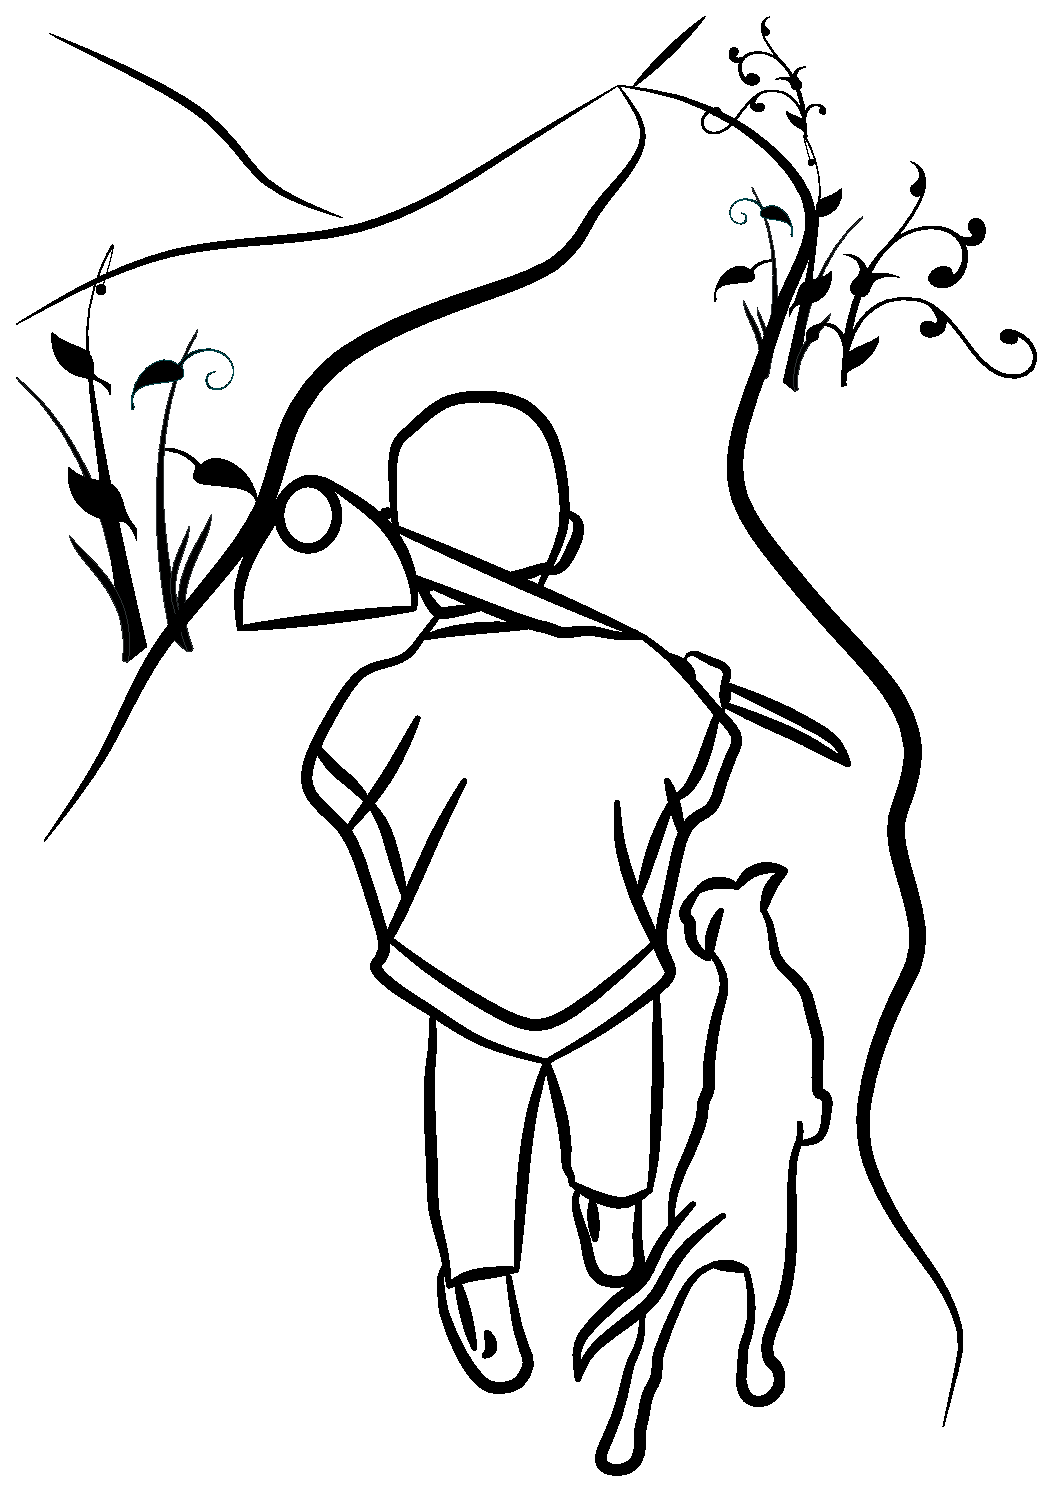
\includegraphics[width=0.47\textwidth]{caminhando.eps}
  \end{center}
  \vspace{-20pt}
  %\caption{Zandor}
\end{wrapfigure}
\fi
Quando era criança, minha família tinha uma cadela que se chamava Zorra, ela era de caráter gentil e muito amorosa com todos nós; meu pai e eu gostávamos de andar com ela para todos os lados. Em algumas ocasiões, durante nossas caminhadas, nós avistávamos a algum conhecido ou familiar, e eles se dirigiam a meu pai falando a viva voz:\\\indent 
--- Bom dia Don Juande!\\\indent
Ele respondia entusiasmado essas saudações com a mesma alegria e energia.
Meu pai na verdade se chamava Juan de Dios\footnote{João de Deus}; porém, carinhosamente, todo mundo preferia chamá-lo de Don Juande.

Eu provavelmente teria cinco ou seis anos nessa época e me lembro de forma clara como minha cadela ia correndo de forma ágil diante de nós, abrindo-nos o caminho através dos montes, latindo e sorrindo.
Estas caminhadas eram muito comuns, uma vez que tínhamos que levar comida para as vacas, procurá-las quando alguma se perdia, ou fazer algum tipo de manutenção à chacra.
No princípio eu não percebi que minha cadela tinha alguns maus costumes, pois com ela nós convivíamos e andávamos de dia, e seu comportamento era irrepreensível. 

\ifdefined\EnableIncludeImages
\begin{wrapfigure}{r}{0.42\textwidth}
  \begin{center}
  \vspace{-30pt}
    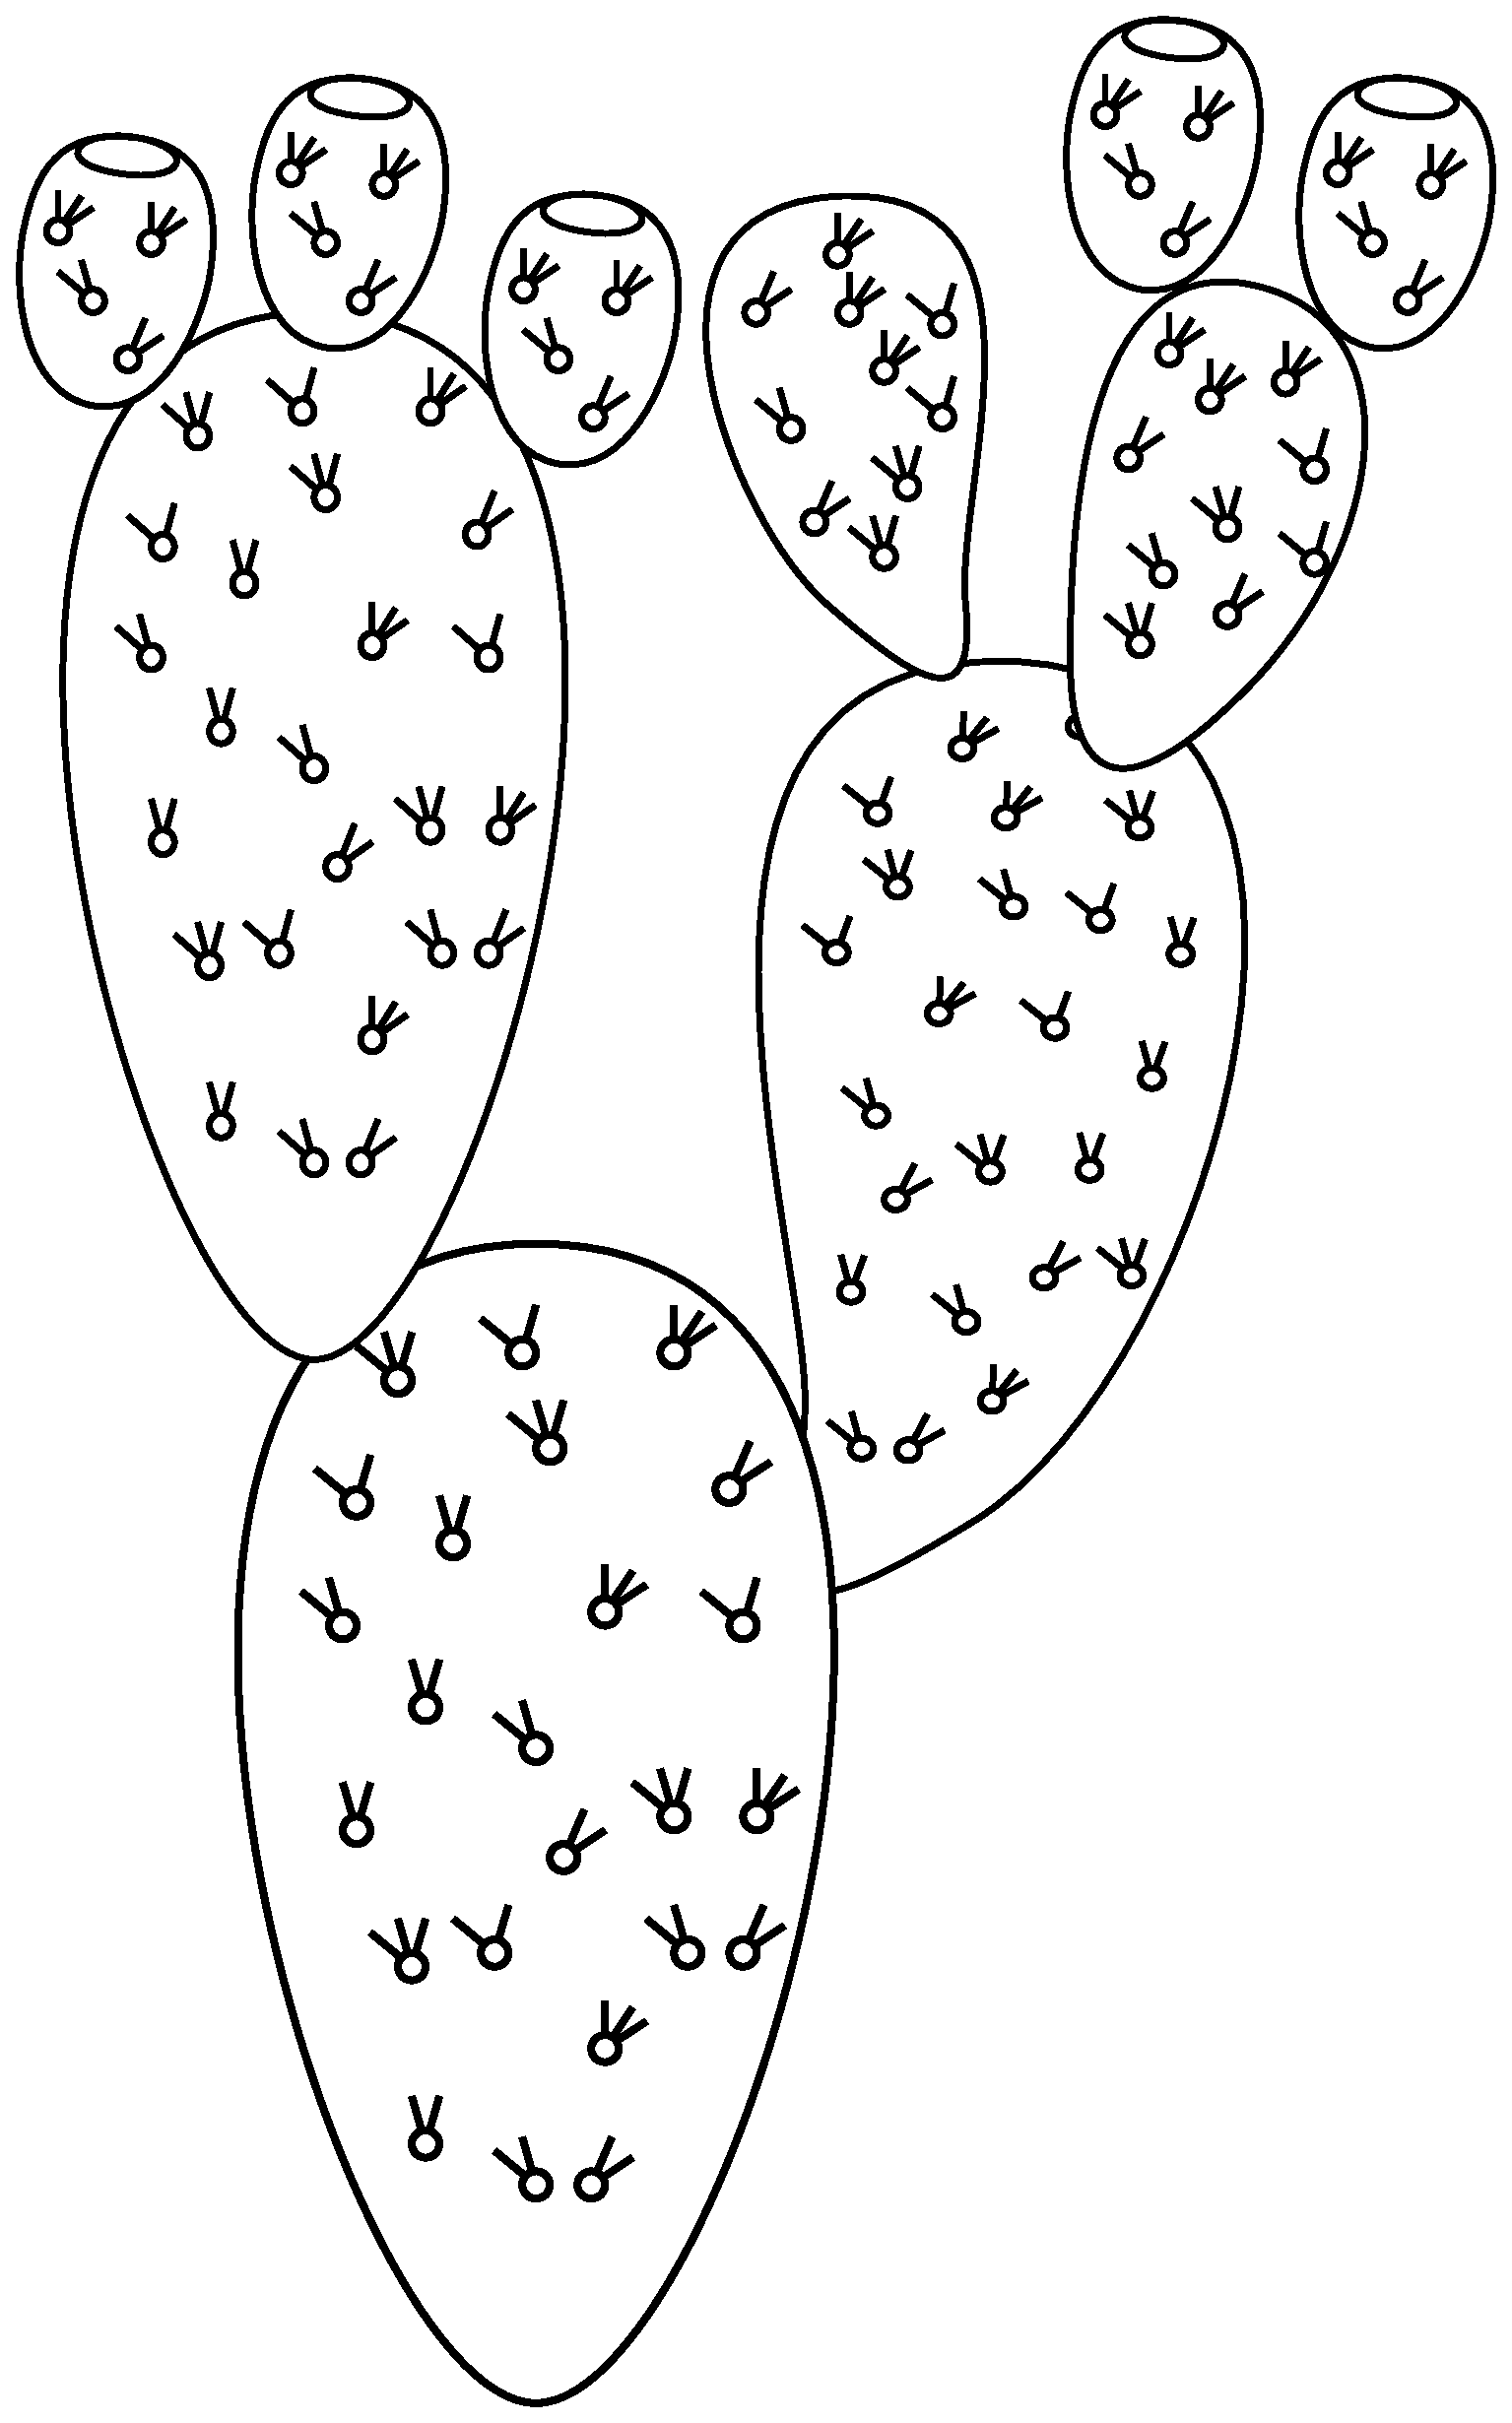
\includegraphics[width=0.3\textwidth]{opuntia.eps}
  \end{center}
  \vspace{-20pt}
  %\caption{Figo das índias.}
\end{wrapfigure}
\fi
Ainda me lembro da primeira vez que fui ao rio acompanhando meu pai e Zorra. Minha mãe tinha encarregado a ele, com caráter de urgência, a missão de obter alguns peixes para serem fritos no almoço; eu rapidamente me uni a tão nobre encomenda, pois gostava de sair a andar. 
Para chegar ao rio, nós tivemos que descer uma ladeira através de um caminho cercado de plantas de figos-da-índia. Quando chegamos lá, eu vi que as margens das águas estavam cheias de juncos\footnote{É um grupo de plantas semelhantes às gramíneas que geralmente crescem nos alagadiços.}, sendo esse um lugar ótimo para explorar e brincar. Assim, enquanto meu pai pescava, minha cadela e eu procurávamos ninhos com ovos de perdiz, sem embargo, Zorra sempre os achava primeiro, comia tudo, ou quase tudo, e eu só conseguía salvar alguns para mim.


Dessa forma passaram-se alguns anos, nos quais ninguém chegou à nossa casa trazendo alguma reclamação ou comentário sobre Zorra; porém um dia entrei na horta que estava próxima à minha casa e fiquei surpreendido ao achar vários pequenos ``tesouros'' dentro de um esconderijo. Havia uma sacola de tecido com pão, outra com açúcar, uma com doces e algumas pequenas ferramentas espalhadas. 
Para mim tudo isso era inacreditável, pois nós só tínhamos coisas como açúcar ou bolachas quando meu pai voltava de suas viagens após trabalhar quatro meses em Ica ou alguma outra cidade grande.
Num primeiro momento, a alegria invadiu meu coração, não obstante, lembrei que meu pai era uma pessoa muito rigorosa, não gostava pegar as coisas dos outros, e dizia:\\\indent
--- Se você encontrar alguma coisa no caminho, no campo, ou na pampa, você não deve pegar ---
e ele agregava:
--- Seguramente alguém o deixou cair, a pessoa que perdeu vai voltar a procurar, e se você leva, ela não vai encontrar.\\ 

Eu lembrava muito bem desse ensinamento, porque uma vez, quando eu estava na solidão do campo pastando as minhas vacas, achei uma ferramenta para fazer fios de lã, que no meu povoado chamávamos de ``callapa''\footnote{Também chamado fuso, este é um utensílio cilíndrico feito geralmente de madeira, utilizado para fiação e torção de fibras como lã.}; provavelmente a ferramenta era de algum outro pastor que passou por ali, mas naquele momento não pensei nisso, só peguei a callapa e retornei à minha casa; já na tarde, cheguei  muito contente, falando:\\\indent
--- Mamãe, papai, olhem o que achei no campo!\\\indent
Meu pai imediatamente respondeu:\\\indent
--- Aqui não tem nada para ser encontrado! Isso é de alguém, alguma pessoa perdeu e ela vai ir a procurar. Volte e deixe isso onde você achou.

\ifdefined\EnableIncludeImages
\begin{wrapfigure}{r}{0.42\textwidth}
  \begin{center}
  \vspace{-10pt}
    
\includegraphics[width=0.4\textwidth]{tools-spindle.eps}
  \end{center}
  \vspace{-20pt}
  %\caption{Figo das índias.}
\end{wrapfigure}
\fi
Nesse momento, um frio desceu desde o topo da minha cabeça até as pontas dos meus pés, pois já quase eram as seis da tarde, tudo estava obscuro, as poucas luzes eram muito distantes e vinham apenas das casas dos vizinhos --- isto era assim porque lá na serra, nessa época, as famílias moravam em casas distanciadas cerca de uns 200, 300, 400 metros umas das outras, ou algumas vezes até mais ---, e para finalizar, eu era muito medroso no que se referia a lugares obscuros e onde tinha que ir estava muito longe.

Diante da ordem do meu pai, eu fui correndo e chorando naquela direção. No caminho não podia distinguir as coisas a alguns metros de mim, porque a lua era minguante; entretanto, quando estava quase na metade do meu destino e meu caminhar era cada vez mais hesitante, observei as sombras ao meu redor, e numa trilha paralela à minha, entre pedras e árvores grandes, vi a silhueta do meu pai me seguindo às escondidas e a uma distância significativa.
Com essa certeza no meu coração, eu segui meu caminho com um pouco mais de tranquilidade, pois sentia que meu pai estava cuidando de mim; mesmo assim, eu seguia chorando de medo, porque na serra, a noite é densa e absoluta, e os sons do caminho alimentavam facilmente a imaginação de uma criança.
No último terço do caminho, eu decidi ir correndo, já que sentia que não podia aguentar mais essa situação. Por fim, cheguei ao meu destino, joguei a callapa no exato lugar onde tinha achado e rapidamente empreendi o caminho de retorno.
Na volta, também senti a presença do meu pai a alguns metros de mim, ou pelo menos eu queria acreditar isso. Com essa seguridade cheguei à minha casa em menos tempo do que gastei para ir, no entanto, quando entrei, meu pai estava sentado lá como se nada tivesse acontecido.


Por essa velha experiência, e tendo a certeza da autoria de Zorra, já que esse esconderijo era o seu lugar favorito, eu tive muito medo por ela, pois sabia que meu pai não iria gostar que Zorra estivesse pegando as coisas de outras pessoas; pelo que, se eu avisava a ele, meu pai iria castigá-la severamente. Por esse motivo decidi não dizer nada sobre minha descoberta, entretanto, tenho que reconhecer que: além do amor pela minha cadela, também pesou na minha decisão que o lugar estivesse cheio de açúcar, pão e outras coisas, que para nós, gente da serra, eram considerados luxos. 
Por esse motivo decidi passar por ali antes de ir à escola ou à chacra: para comer bolachas, água com açúcar, ou qualquer outra coisa boa que estivesse por ali. 
Para meu desespero, um dia Zorra trouxe demasiadas coisas, eu  não podia imaginar de onde havia pegado tudo aquilo, já que ela só ``trabalhava'' durante à noite, enquanto todos nós dormíamos. Assim, diante daquele aumento na criminalidade que largamente desbordava seu esconderijo, meu pai descobriu toda a situação.
Muito para meu pesar, ele a castigou severamente, desde minha casa eu somente escutei seus lamentos recebendo a punição, pois eu preferi não ver.


Depois dessa experiência, ela deixou de levar as coisas à horta, e o problema parecia resolvido. Porém, logo descobriríamos que longe da casa, numa pedra grande e obscura, perto da casa de um vizinho, 
Zorra havia reiniciado suas atividades. Assim, de dia, diante dos olhos da família, se comportava como uma cadela exemplar. Porém, durante a noite, ela roubava dos vizinhos as mais variadas coisas.

\ifdefined\EnableIncludeImages
\begin{wrapfigure}{r}{0.42\textwidth}
  \begin{center}
  \vspace{-10pt}
    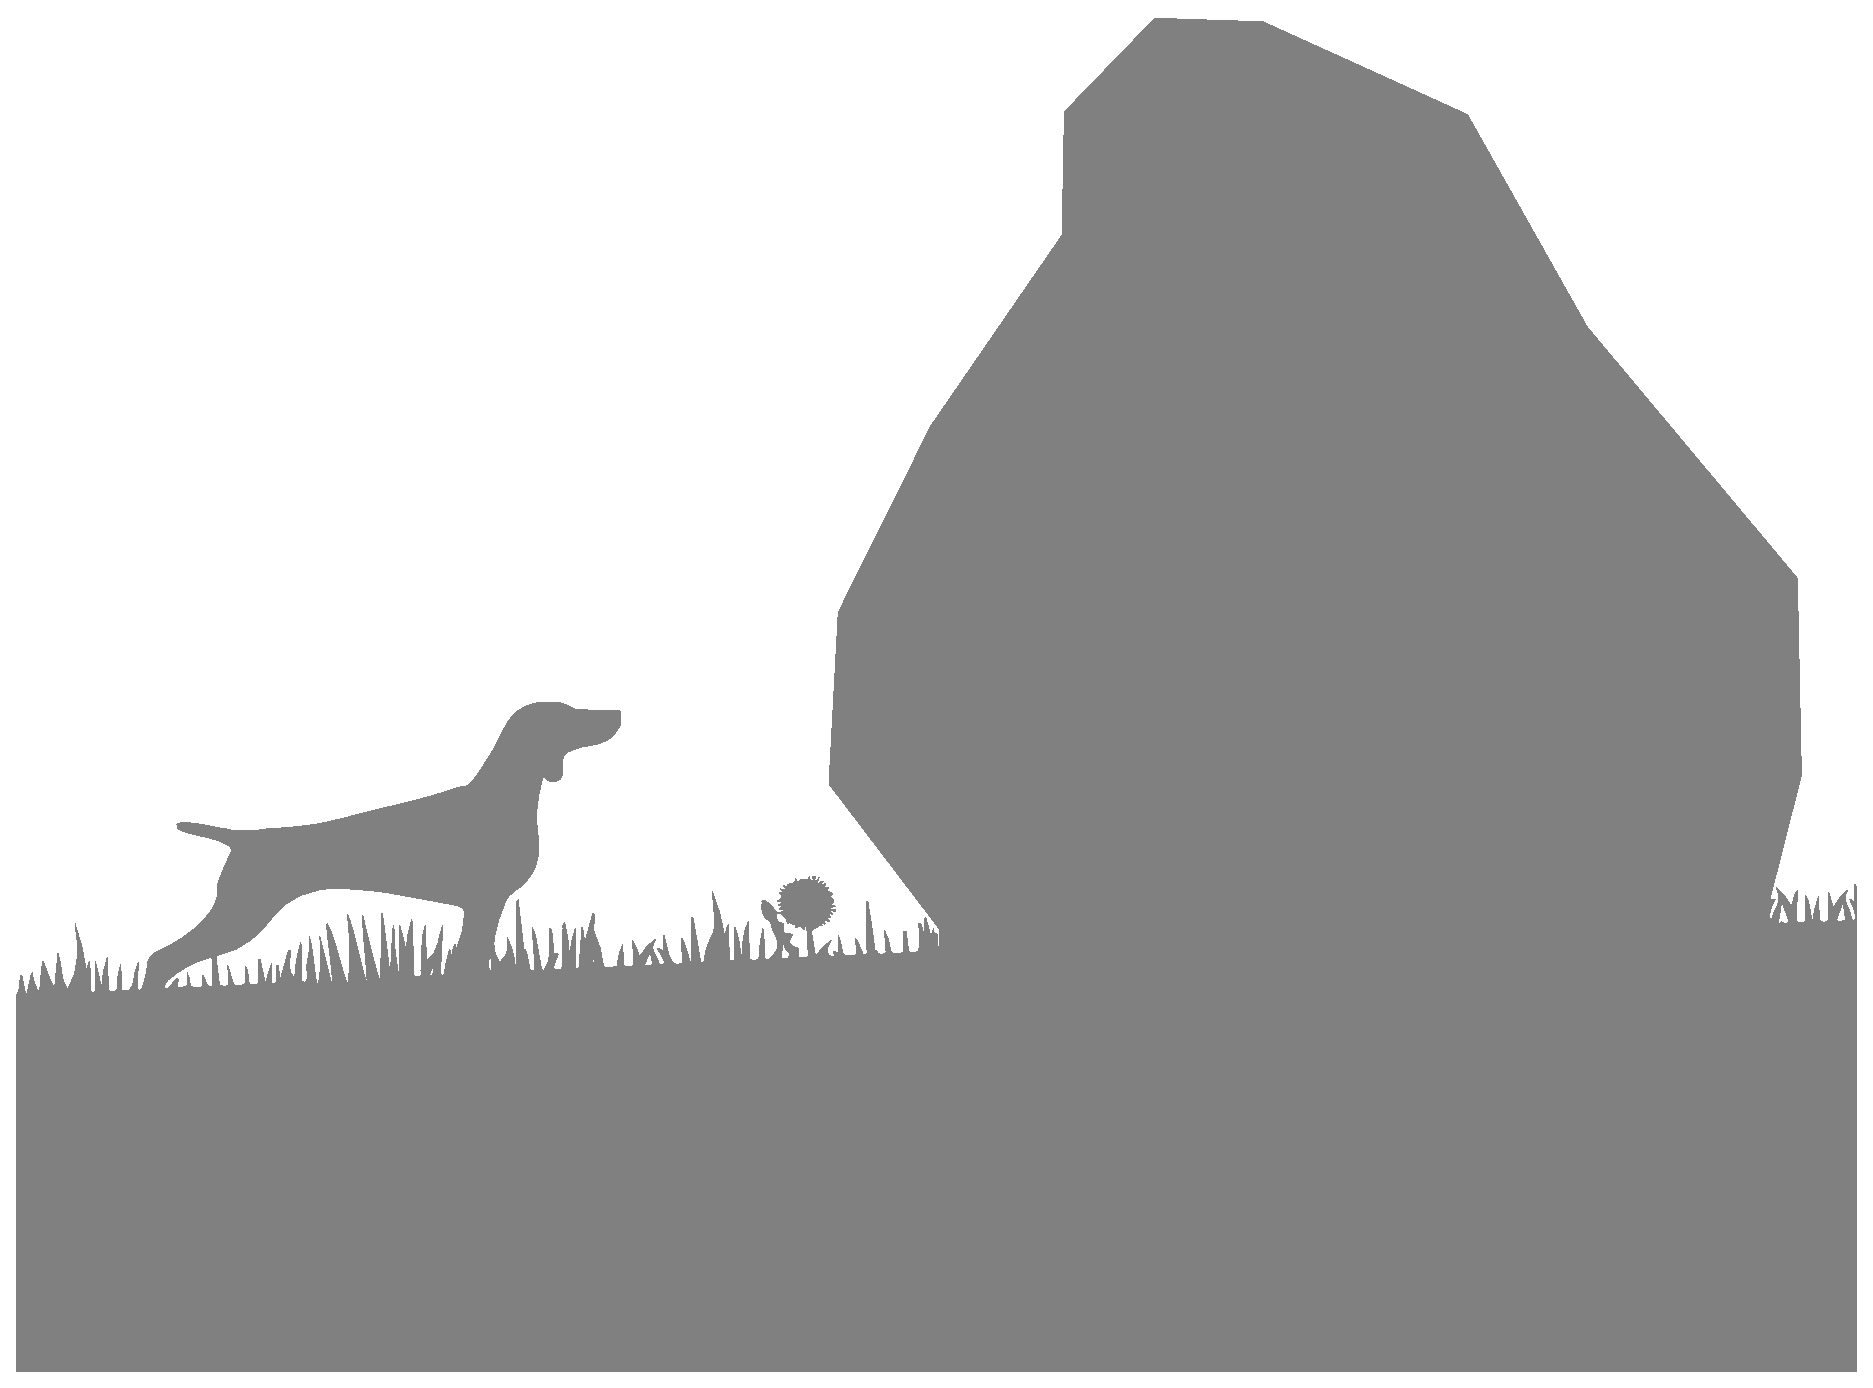
\includegraphics[width=0.4\textwidth]{zorra-rock.eps}
  \end{center}
  \vspace{-20pt}
  %\caption{Figo das índias.}
\end{wrapfigure}
\fi
Nesse momento foi a primeira vez que uma pessoa chegou a minha casa para fazer uma reclamação. O pagante denunciou que ele viu pessoalmente como Zorra havia entrado na sua casa para roubar. 
A indignação do meu pai foi tão grande quanto sua vergonha, pois não foi um vizinho ou algum familiar nosso, que poderia entender a situação, mas sim uma vítima que morava muito longe de nós, em outro povoado, que foi perguntando entre os vizinhos até achar primeiro suas coisas e logo nossa casa.
Nessa ocasião meu pai castigou mais severamente a Zorra; diante dessa difícil situação, minha maior tristeza era que eu já compreendia que esse problema não ia a solucionar-se com outro castigo, e minhas dúvidas foram confirmadas quando percebi que Zorra seguia saindo de noite. 

Muito tempo depois descobriríamos que Zorra novamente tinha mudado de esconderijo e que levava suas coisas a outra pedra grande, perto da casa de uma vizinha que era viúva e que carinhosamente chamávamos avó Mesla --- na verdade, ela não era familiar nosso, mas o costume na serra era chamar avó a qualquer pessoa de idade, como sinal de respeito, já que vivíamos com eles como se fossem de nossa família ---.
Assim, antes que alguma pessoa da minha casa conhecesse esse novo lugar, no qual Zorra ocultava seus objetos roubados, outra pessoa chegou a denunciar novamente a cadela, e mesmo que meu pai castigou, gritou e tentou segui-la, não conseguimos achar o novo esconderijo. Assim, o tempo passou sem que essa incógnita fosse resolvida. 

Um dia meu pai, minhas irmãs e eu decidimos descer ao rio para pescar, porém esse dia não achamos a Zorra para que nos acompanhasse. Transcorreu o dia e quando eram as quatro ou cinco da tarde, nós estávamos prontos para regressar a casa com a pesca do dia. Nesse momento, eu escutei um ruído entre os juncos do rio, onde costumava brincar com Zorra, por pura curiosidade fui averiguar o que era aquele som similar a um choro agudo. Para minha surpresa, lá estava sozinho um cachorro pequeno e pretinho que minha cadela havia parido.  
Para que meu pai não visse ele, eu escondi o filhote dentro do meu agasalho, já que desconfiava que ele me deixasse levar um novo cachorro a casa, pois os problemas que Zorra gerava já eram suficientes para nós, como para arriscar mais a reputação da família com outro cachorro.
Só quando cheguei em casa tirei o cachorro de dentro das minhas roupas e diante das minhas irmãs, minha mãe e meu pai, apresentei o novo membro da família. Dado que naquela época, minhas irmãs estavam aprendendo a ler usando um livro chamado ``Lola e Pepe'', onde nas suas histórias descreviam a um cachorro chamado Zandor, eu decidi usar esse nome para meu novo cachorro. 

Assim, mesmo com seus novos deveres de mãe, Zorra não deixava de causar problemas, já que aos nossos ouvidos chegavam histórias de roubos em povoados distantes, e as ausências de Zorra se volviam cada vez mais prolongadas.
Para nossa má sorte, num povoado vizinho, tinha-se espalhado a notícia que era uma cadela a responsável de todos os roubos, e, num triste dia, os moradores dessa localidade se organizaram, entre todos conseguiram encurralá-la e capturá-la, e finalmente, sob o abrigo da massa e sem nenhum remorso, deram morte a minha querida Zorra.
Esse mesmo dia chegou na minha casa a notícia da sua morte... entre lágrimas e lamentos fomos a esse povoado para enterrar a nossa querida cadela, já que nos informaram que eles simplesmente tinham jogado seu corpo na beira do rio. Quando chegamos lá, a encontramos gelada e inerte, e instintivamente a embrulhamos num tecido, como se fosse um bebê, para que não passasse frio... ao seu lado choramos até que as nossas lágrimas se secaram, pois ela tinha sido nossa amiga fiel, e mesmo que soubéssemos de  seus maus costumes, nós a amávamos.
Nesse mesmo lugar, ao finalizar o dia e com o rio como testemunha, fizemos uma pequena cerimônia e enterramos a quem em vida foi conhecida por nós como Zorra. 

No dia seguinte, a notícia já tinha se espalhado pelo meu povoado, e mesmo que nós assumíamos que não receberíamos condolências de parte dos vizinhos, para nos desenganar, a avó Mesla chegou chorando à porta de nossa casa e entre seus lamentos dizia:
\begin{quotation}
\noindent ``Eu não tinha panela, e \\Zorra me levou uma panela;\\ 
eu não tinha frigideira, e \\Zorra me levou uma frigideira;\\ 
eu não tinha colher, e \\Zorra me levou uma colher;\\
eu não tinha faca, e \\Zorra me levou uma faca;\\
quando tive fome, \\Zorra me levou pão...''
\end{quotation}
Minha mãe a abraçava, enquanto avó Mesla continuava com sua litania, por aquele animal que, a seu modo de ver, só tinha chegado a sua vida para ajudá-la no seu momento de maior necessidade.
 



%----------------------------------------------------------------------------------------
%	CHAPTER TWO
%----------------------------------------------------------------------------------------

\cleardoublepage
\newpage
\ifdefined\EnableIncludeImages
    \ThisULCornerWallPaper{1.0}{chapterimage.eps}
\fi
\chapter{Zandor}

Após a morte de Zorra, toda a família ficou muito triste, pois apesar de seus maus costumes, ela sempre foi muito amorosa conosco; por isso, sentíamos sua falta como se fosse um membro da família. 
Assim, passamos muito tempo chorando, sobretudo minhas irmãs e eu, que ainda éramos crianças. 
Muitas vezes vi a Teodosia ---  minha irmã mais velha, a qual carinhosamente chamávamos ``Tulaco'' ---, iniciar a chorar em silêncio ao ver o lugar onde Zorra dormia; inclusive Diofelia  --- ``Dio'', a minha irmã mais nova ---, apesar de sua curta idade, já sabia distinguir a morte e a ausência que ela deixa. 
Eu também chorava, talvez mais do que elas, porque Zorra era minha companheira fiel, ela me seguia em todos os lugares onde eu ia; pois, ao ser o filho homem da casa, eu era quem tinha que sair para trabalhar na chacra com meu pai, e Zorra sempre fazia mais alegres e memoráveis esses momentos.
Nosso único conforto era que tínhamos o Zandor; nós o amávamos por ser o último presente que Zorra nos deixou.
Eu olhava para Zandor --- todo pequeno e pretinho --- e ficava maravilhado com o quanto era fofo. Sua presença me dizia que, de alguma forma, uma parte de Zorra ainda estava conosco. 
Assim, Zandor cresceu sendo criado com muito cuidado e carinho por todos nós;
entretanto, a personalidade de Zandor era completamente distinta da de sua mãe; ele era um cachorro muito honesto e era evidente para nós que ele não tinha nenhuma dos maus costumes de Zorra. 
\ifdefined\EnableIncludeImages
\begin{wrapfigure}{r}{0.45\textwidth}
  \begin{center}
  \vspace{-20pt}
    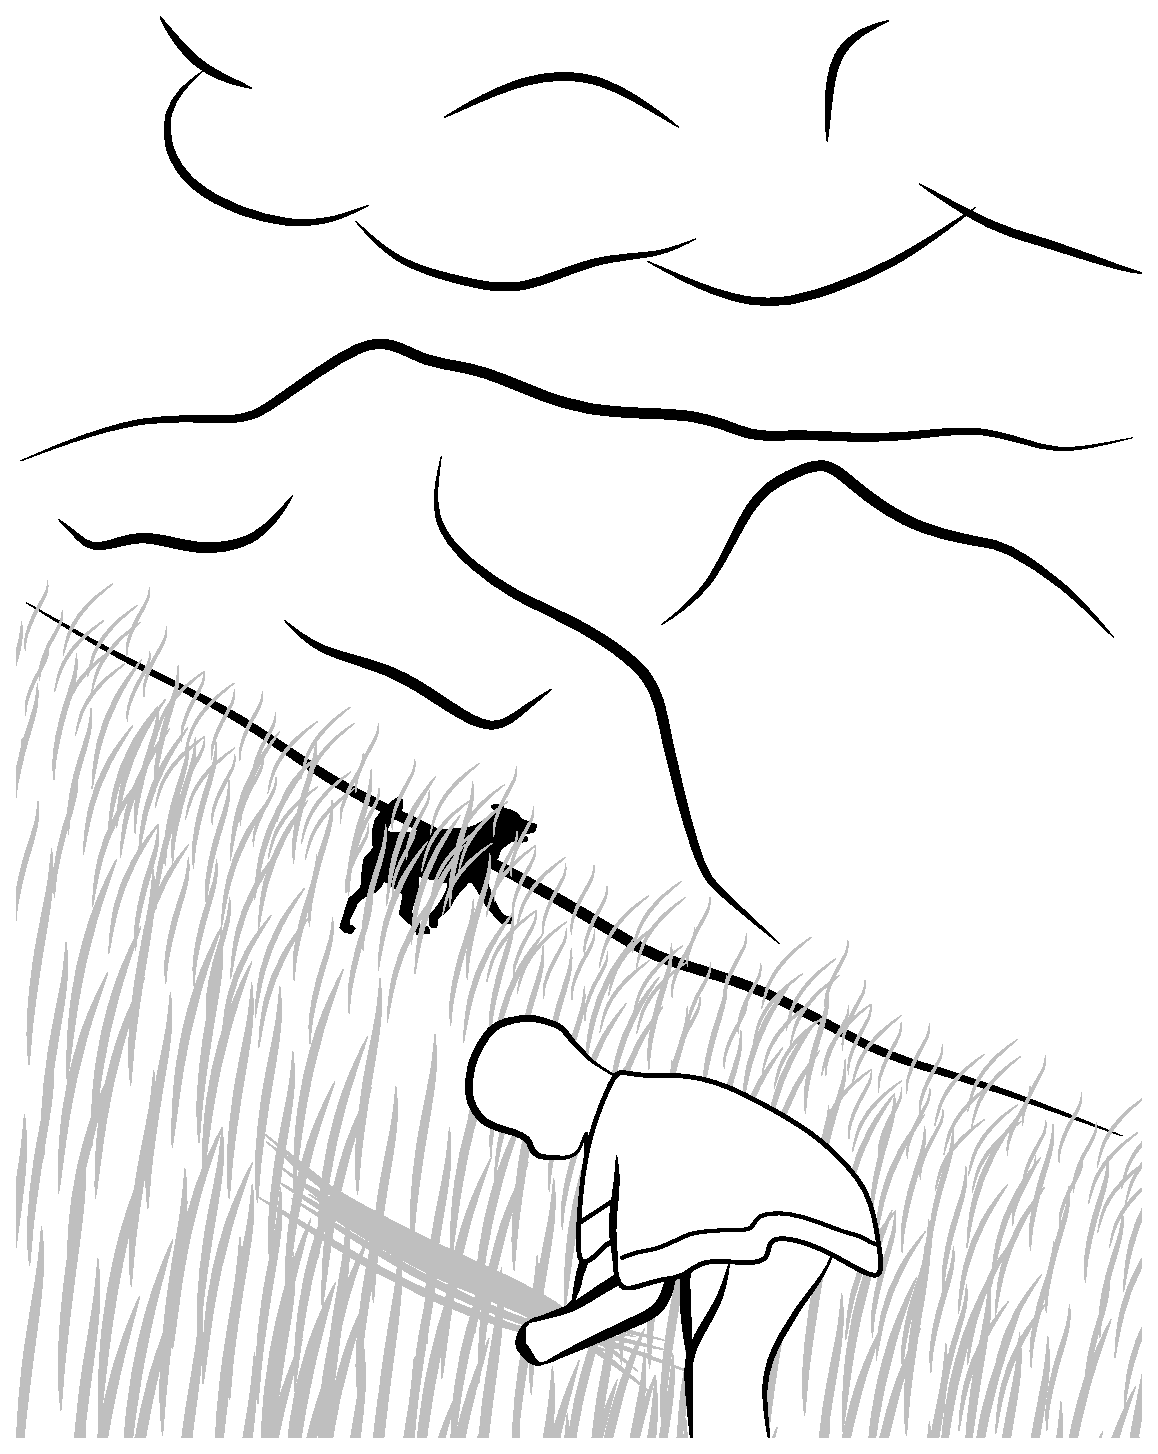
\includegraphics[width=0.43\textwidth]{pasto-zandor-aulicha}
  \end{center}
  \vspace{-20pt}
  %\caption{Figo das índias.}
\end{wrapfigure}
\fi
Desde pequeno eu levava Zandor a todas as minhas caminhadas pelo campo; como minha família tinha vacas, eu tinha que ir dar-lhes comida e atendê-las, e comumente recompensava Zandor por sua companhia dando-lhe leite fresco, que eu mesmo ordenhava para matar a nossa fome. 
Com todos esses cuidados, em pouco tempo Zandor virou um cachorrinho forte e muito brincalhão.
Ele me ajudava a cuidar das vacas e assustava os pássaros que vinham comer as sementes na chacra. Quando eu gritava seu nome, ele vinha correndo e se parava de frente a mim com a severidade de um soldado diante do seu general; ele era tão inteligente quanto uma pessoa e bem mais obediente que eu mesmo.

Um dia, quando estava no campo com Zandor, observamos que uma perdiz saía voando de uns arbustos. Para Zandor, que ainda era filhote, foi a primeira vez que ele viu uma perdiz; eu, pelo contrário, já tinha experiência com essas aves e sabia que próximo a esse lugar acharíamos um ninho, ovos ou crias. 
Automaticamente, gritei:\\\indent
--- Zandor! Vamos buscar ovos!\\\indent
Ele latiu ao sentir minha empolgação e avançou junto a mim na direção que eu indiquei para ele. 
Era gostoso ver Zandor, pequeno, porém corajoso, batendo seu rabinho, cheirando para todos os lados, levantando e recolhendo suas orelhas; como se, naquela primeira missão de busca, quisesse demonstrar sua eficácia usando ao máximo todos seus sentidos. 
Só procuramos uns minutos e de repente os vimos\\\indent
--- Olha Zandor! Ovos! --- gritei.\\\indent
Ele latiu como afirmando minha exclamação, e me acerquei ao ninho para recolher todos os ovos. Zandor não pegou nenhum, ele só me olhava contente enquanto eu os colocava num saquinho de tecido para protegê-los e levá-los a casa. 


Esse procedimento se tornou comum, e cada vez que eu saía para procurar as nossas vacas, também aproveitava para procurar ovos de perdiz com Zandor; quando os achávamos, eu os levava muito contente para minha mãe; de modo que, todos os dias, nós voltávamos com 8, 12 ou até 15 ovos. 
Com o passar dos meses, Zandor virou um especialista em encontrar ovos, pois ele já não era um filhote, e eu não precisava acompanhá-lo mais. Assim, enquanto eu trabalhava, ele saía por conta própria a procurar ovos; no instante em que ele os achava, latia repetidas vezes e sem descanso, até chamar minha atenção, de modo que minha única missão era recolhê-los e levá-los para casa.
\ifdefined\EnableIncludeImages
\begin{wrapfigure}{r}{0.43\textwidth}
  \begin{center}
  \vspace{-20pt}
    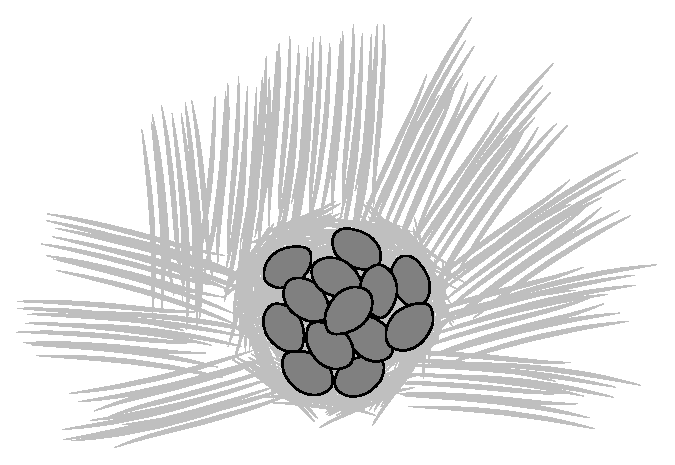
\includegraphics[width=0.40\textwidth]{huevos.eps}
  \end{center}
  \vspace{-20pt}
  %\caption{Figo das índias.}
\end{wrapfigure}
\fi
Algumas vezes, cozinhávamos os ovos, outras vezes os fritávamos; e numa dessas ocasiões, meu pai chegou em casa quando estávamos cozinhando-os,\\\indent
--- e esses ovos?--- perguntou ele, 
e eu, contente e cheio de orgulho, respondi:\\\indent 
--- Zandor achou!\\\indent
Ele meditou um pouco e replicou:\\\indent 
--- Zandor achou... e que coisa deram a ele?\\\indent
A pergunta me pegou de surpresa e falei em voz baixa:\\\indent 
--- Nada pai, só a comida da casa... \\\indent
Meu pai me olhou e falou calmamente: \\\indent
--- Se foi ele quem achou, ele também deve participar.\\\indent
Nesse momento meu pai pegou um ovo cru e deu para o cachorro, Zandor pegou contente o ovo e lambeu até sobrar só a casca. A partir de então, Zandor se acostumou a comê-los sempre que lhe ofereciam. 
Assim, cada vez que ele encontrava ovos, eu os levava para casa, os entregava a minha mãe e ela por sua vez entregava dois a Zandor; porém, nunca lhe dávamos os ovos quando ele os encontrava, somente na casa, ele por sua parte sabia esperar e nunca pegou nenhum, só esperava pacientemente o momento que minha mãe entregasse a ele seus ovos e ia contente a seu cantinho para comê-los.


Para mim, Zandor era maravilhoso, em qualquer lugar aonde eu ia, ele me acompanhava, quando estava triste ele se sentava a meu lado e até chorava comigo fazendo um som agudo, que eu sentia cheio de solidariedade. 
Por outro lado, se ele percebia que eu estava contente, levantava suas orelhinhas e iniciava a pular e correr de um lado a outro. Assim, durante muito tempo, andamos e crescemos juntos... o tempo passou e eu completei oito anos, e logo, nove anos de idade.

Um dia meu pai decidiu abater um boi; lá na serra não se mata um boi sem nenhum motivo, só em ocasiões importantes como festas regionais, casamentos ou eventos semelhantes. No entanto, eu sabia que nessa época não tínhamos nenhuma festividade e pensava que a meu pai simplesmente ocorreu-lhe abater o boi sem nenhum motivo, mas não era assim. 
Eu tinha um irmão mais velho que morava na capital, em Lima; eu não o conhecia, só sabia de sua existência, pois meus pais sempre falavam sobre sua vida lá e se referiam a ele como ``Seve''; nessa época, eu pensava que ele se chamava dessa forma, não obstante, esse não era seu nome e, sim, Severino. Eu não o conhecia porque viajou para Lima quando eu era muito pequeno, seguramente o vi nessa época, mas eu não tinha lembrança alguma. 
Assim, meu pai e minha mãe tinham a intenção de fazer charque para mandar-lhe como encomenda; com essa finalidade, decidiram abater o boi e prepararam cuidadosamente sua carne com muito sal.

\ifdefined\EnableIncludeImages
\begin{wrapfigure}{r}{0.49\textwidth}
  \begin{center}
  \vspace{-20pt}
    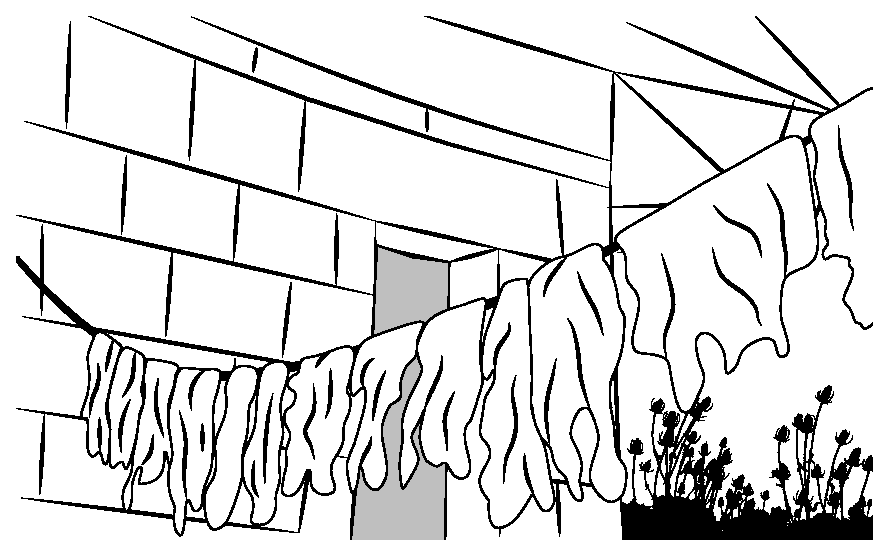
\includegraphics[width=0.47\textwidth]{charque.eps}
  \end{center}
  \vspace{-20pt}
  %\caption{Zandor}
\end{wrapfigure}
\fi
Nosso lar estava composto por uma casa pequena e uma grande, ambas separadas por vários metros entre si; nossa família morava na casa grande e usávamos a pequena para guardar ferramentas, grãos e, em geral, alimentos não perecíveis. 
Perto da casa pequena, nós tínhamos duas figueiras; nesse dia meu pai usou uma delas para amarrar uma corda até a casa pequena, e sobre ela pendurou a carne para secar com o sol; porém, ele decidiu pendurar uma perna de boi no tronco da outra figueira, pois essa peça de carne pesava muito.
Lá o costume é recolher a carne e levá-la para a casa durante a noite, para que os animais de hábitos noturnos não viessem para comê-la, de modo que no dia seguinte, pela manhã, com os primeiros raios do sol, a carne era novamente pendurada; não obstante, nesse dia meu pai recolheu só o charque que estava pendurado na corda e esqueceu a perna que tinha colocado na outra figueira. 
O pior foi que ali, onde meu pai deixou a carne, tranquilamente qualquer cachorro, zorro, ou outro animal carnívoro da serra, poderia pegá-la facilmente, sem a necessidade de pular, uma vez que não estava a muita altura.

Essa noite Zandor não parou de latir; nós, na casa grande, só escutávamos seu barulho com curiosidade, dado que nenhum membro da família lembrou da perna pendurada na figueira. 
Pelo barulho, só reconhecíamos que algumas vezes chegavam outros cachorros, outras vezes não escutávamos nenhum outro animal, só o Zandor latindo com muita raiva e força; meu pai, bravo pelo ruído, só falava:\\\indent
--- Que coisa quer esse cachorro que não nos deixa dormir!\\\indent
Porém, ele não saía da casa grande para indagar sobre a situação. 
Eu tinha muito medo por tudo o que estava acontecendo; pois, na serra, contam histórias dos seres que habitam a noite. 
Alguns diziam que à noite anda o ``cuco''\footnote{Também chamado coca ou coco, este é um ser mítico, uma espécie de fantasma, bruxa ou bicho-papão que anda de noite pelos caminhos.}, e as crianças tinham um terror extremo a esse ser; para piorar a situação, meu pai tinha o costume de contar-nos histórias sobre suas viagens, de como à noite achou o ``cuco'' nos caminhos da serra, ou também que, em algum povoado perto, o ``cuco'' tinha matado algum vizinho, que tinha chupado o sangue de outro ou simplesmente assustado algum caminhante noturno. Devo reconhecer que apesar do terror que me causavam as histórias do meu pai, eu gostava de conhecê-las e passar medo ouvindo-as; ele sempre me contava suas aventuras de quando saía para trabalhar em outras cidades e das coisas que viu, dos problemas que aconteciam no caminho e dos personagens que apareciam quando ele se deslocava a pé.

\ifdefined\EnableIncludeImages
\begin{wrapfigure}{r}{0.49\textwidth}
  \begin{center}
  \vspace{-20pt}
    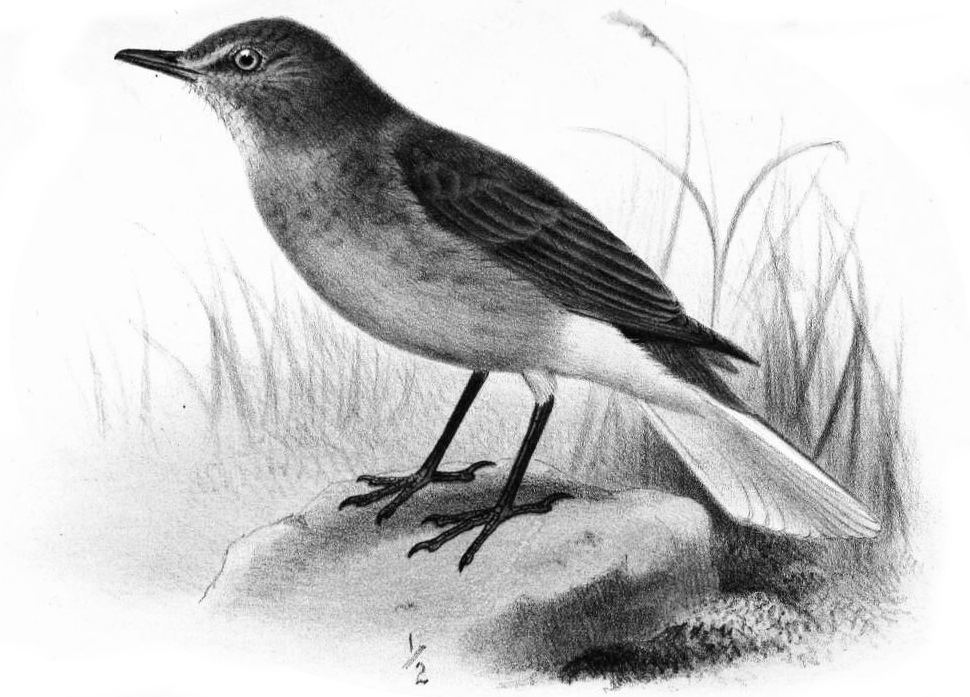
\includegraphics[width=0.47\textwidth]{AgriornisSolitariaSmit.jpg}
  \end{center}
  \vspace{-20pt}
  %\caption{Zandor}
\end{wrapfigure}
\fi
Por exemplo, um dia meu pai me contou que quando estava viajando, caminhando desde nosso povo até ``Cangallo'', um povoado distante, no meio do caminho, a noite chegou, e ele iniciou a procurar entre os trilhos alguma casa que pudesse dar-lhe pousada. Enquanto ele estava nessa tarefa, escutou um pássaro ao qual nós na serra chamamos ``huaychao''\footnote{Também escrito como waychaw, esta é uma palavra quéchua que significa: avisar, anunciar, advertir ou notificar. ``Huaychao'' é uma onomatopeia do som que faz a ave cujo nome científico é Agriornis montanus.}, cujo canto é de mau augúrio.
Meu pai falava que quando o ``Huaychao'' canta, é porque o mal está perto, que ele canta porque viu o mal andando, talvez na forma de algum ``jarjacha''\footnote{Também chamado carcaq ou qarqacha.}. 
Para nós, os ``jarjachas'' são seres da noite, são pessoas que se levantam dos seus túmulos, pois ao terem feito coisas terríveis em vida, estão condenadas a não morrer e vagar de noite entre o sofrimento e a ira. 
Então, meu pai sempre me advertia muito sério que, se na noite escutava ao huaychao, devia ter muito cuidado porque seguramente um ``jarjacha'' estava perto. 
Na sequência dos fatos, quando meu pai escutou ao huaychao, começou a correr pulando pedras e atravessando riachos até que, só e assustado, achou uma casa; rapidamente bateu à porta e de dentro, escutou uma voz de mulher que lhe perguntava:\\\indent
--- Boa noite! Quem está aí?\\\indent
Meu pai, todo assustado, tentou lhe explicar que era só um viajante, que a noite tinha chegado na metade do seu caminho e que somente precisava de um lugar para dormir. A senhora, do interior da casa, respondeu-lhe que, da mesma forma que ele falou, seres que não são pessoas, ``cucos'', andam pela noite enganando os moradores para conseguir entrar em suas casas,\\\indent
--- de repente você é um deles! --- Disse a senhora e negou a meu pai um lugar para dormir.\\\indent
Ele insistiu com a voz tremida pelo medo, porque sabia que tudo isso era verdade, pois ele já tinha escutado ao huaychao e sabia que o mal estava perto. Por fim, após discutir muito, a senhora se comoveu e deixou a meu pai entrar em casa. 
A senhora, toda curiosa pela situação, perguntou a meu pai por que andava à noite, e ele explicou que só estava tentando ir de Occo até Cangalho; porém, teve problemas no caminho e a noite lhe pegou. 
Imediatamente a senhora respondeu em tom maternal:\\\indent 
--- Por que você anda à noite? Só ontem um ``jarjacha'' comeu uma pessoa, agora esse vizinho está morto, hoje mesmo enterramos ele.\\\indent
Por todas essas histórias, sair da casa grande de noite, só porque o cachorro latia, era uma completa temeridade; até meu pai tinha medo de sair, ele só gritava para Zandor de dentro da casa, segurando sua ``guaraca''\footnote{Corda muito versátil que pode ser usada como cinto de calças ou para disciplinar crianças desobedientes.}, golpeando com ela a parede. 
Os demais membros da família, incluindo-me, só escutávamos resignados, tentando dormir apesar do barulho.

Assim, a noite passou, e praticamente nenhum de nós conseguiu dormir. 
Quando os primeiros raios do sol tocaram a nossa janela, todos nós saímos em direção à casa pequena e, para nossa surpresa, vimos a perna de boi pendurada na figueira. 
Para nós foi evidente que, durante a noite, os animais do campo tinham chegado para comer a carne e Zandor tinha defendido-a, brigando, latindo e sem dormir.
\ifdefined\EnableIncludeImages 
\begin{wrapfigure}{r}{0.47\textwidth}
  \begin{center}
  \vspace{-0.5cm}
    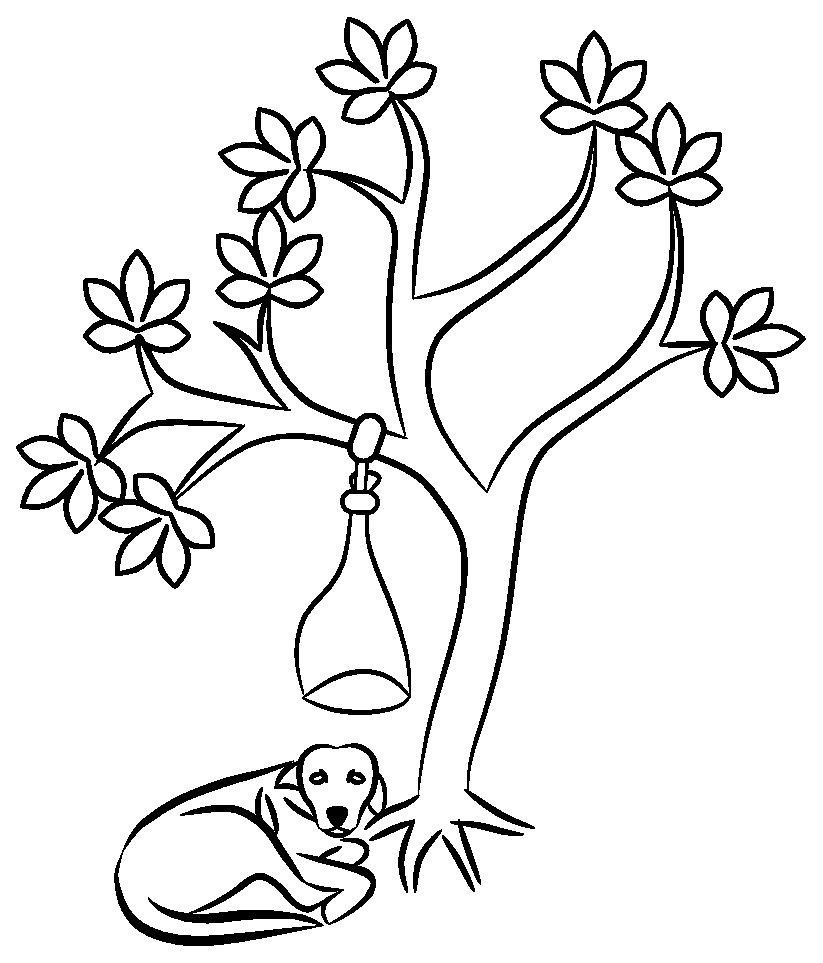
\includegraphics[width=0.45\textwidth]{perro-fiel-1.eps}
  \end{center}
  \vspace{-0.5cm}
  %\caption{Zandor}
\end{wrapfigure}
\fi
Ele estava aconchegado, encolhido em forma de bolinha abaixo da perna de boi e, ao nos ver chegar, só nos dirigiu um olhar cansado enquanto abanava o rabinho. Meu pai se admirou pelo desempenho de Zandor, pois a carne estava intacta.\\\indent
--- Como me esqueci da perna! Por isso chegavam os cachorros! --- exclamou meu pai.\\\indent
Automaticamente entrou na casa, pegou uma faca, cortou um pedaço grande de carne da perna de boi, ainda pendurada na figueira, e a entregou a Zandor como um prêmio; só nesse momento, ele olhou a carne com vontade, pegou seu prêmio e foi para o canto dele para comer.

Assim, Zandor cresceu sendo sempre um cachorro honrado. Se você não dava alguma coisa, ele não pegava; por isso, toda a família o respeitava. Além disso, no campo, os cachorros sempre são bem cuidados; eles comem a mesma comida dos donos de casa e são tratados com carinho, sendo eles considerados como membros da família.



%----------------------------------------------------------------------------------------


%----------------------------------------------------------------------------------------
\backmatter
\chapterwithtocfalse

%----------------------------------------------------------------------------------------
%	COLOFÃO
%----------------------------------------------------------------------------------------
\cleardoublepage

\null
\vfill

\begin{flushright}
{\normalsize \it Continuará.
\vspace*{4pt}}
\end{flushright}

\newpage

\null
\vfill
\thispagestyle{empty}


{\normalsize \it Este livro foi produzido por \myauthor, editado e diagramado usando \LaTeX,
com um tipo de fonte \showfont,
para ser impresso num papel tamanho \imprimirpapersize. Edição criada em \imprimirdata.
\vspace*{4pt}}







%----------------------------------------------------------------------------------------

\end{document}
